\documentclass[tikz,border=1mm]{standalone}

\usepackage{amsmath}
\usepackage{graphicx}
\renewcommand\familydefault{\sfdefault} 
\usepackage[T1]{fontenc}

\usetikzlibrary{arrows,shapes,calc,math,decorations.fractals,patterns,backgrounds,decorations.markings}
\tikzset{every picture/.style={/utils/exec={\sffamily}}}
\tikzset{point/.style={fill,circle,inner sep=1.5pt}}
\tikzset{bluevec/.style={-triangle 45,blue,line width=1pt}}
\tikzset{vec/.style={-triangle 45,blue,line width=1pt}}
\tikzset{redvec/.style={-triangle 45,red,line width=1pt}}
\tikzset{greenvec/.style={-triangle 45,green!50!black,line width=1pt}}
\tikzset{axis/.style={-stealth',line width=1pt}}
\tikzset{dblarrow/.style={latex'-latex',shorten <= 2pt, shorten >= 2pt}}

\tikzset{partial ellipse/.style args={#1:#2:#3}{insert path={+ (#1:#3) arc (#1:#2:#3)}}}

\begin{document}

% 3D axes
% \begin{tikzpicture}
%     \draw [axis] (0,0) -- (330:2) node [below right] {$x$};
%     \draw [axis] (0,0) -- (30:2) node [right] {$y$};
%     \draw [axis] (0,0) -- (90:2) node [above] {$z$};
% \end{tikzpicture}

% 3D cartesian co-ordinates
% \begin{tikzpicture}
%     \draw [axis] (0,0) -- (330:3) node [below] {$x$};
%     \draw [axis] (0,0) -- (30:4) node [right] {$y$};
%     \draw [axis] (0,0) -- (90:3) node [left] {$z$};
%     \draw [dashed] (330:2) -- ++(30:2) -- ++(150:2) -- ++(90:1) -- ++(210:2) -- ++(330:2) -- ++(30:2) coordinate (p) -- ++(150:2) (p) -- ++(270:1) (330:2) -- ++(90:1);
%     \draw [fill] (p) circle (2pt) node [above right] {$(x,y,z)$};
%     \draw [dblarrow] (210:0.2) -- node [below] {$x$} ++(330:2);
%     \draw [dblarrow] (330:2.2) -- node [below right] {$y$} ++(30:2);
%     \draw [dblarrow] ($(p)+(0:0.2)$) -- node [right] {$z$} ++(270:1);
% \end{tikzpicture}

% Vector
% \begin{tikzpicture}
%     \coordinate (s) at (2,0);
%     \draw [axis] (0, 0) -- ++(330:1) node [below] {$x$};
%     \draw [axis] (0, 0) -- ++(30:1) node [right] {$y$};
%     \draw [axis] (0, 0) -- ++(90:1) node [left] {$z$};  
%     \draw [dashed] (s) -- ++(330:2) -- ++(30:2) -- ++(90:1) coordinate (a) (s) -- ++(30:2) -- ++(330:2) (s) -- ($(a)+(270:1)$);
%     \draw [bluevec] (s) -- node [above left,pos=0.75] {$\mathbf{a}$} (a);
%     \draw [dblarrow] ($(s)+(210:0.2)$) -- node [below] {$a_x$} ++(330:2);
%     \draw [dblarrow] ($(s)+(330:2.2)$) -- node [below right] {$a_y$} ++(30:2);
%     \draw [dblarrow] ($(a)+(0:0.2)$) -- node [right] {$a_z$} ++(270:1);
% \end{tikzpicture}

% Vector addition
% \begin{tikzpicture}[auto]
%     \draw [bluevec] (0, 0) -- node {$\mathbf{a}$} ++(45:3) coordinate (a);
%     \draw [redvec, shorten >=4pt] (a) -- node {$\mathbf{b}$} ++(-15:3) coordinate (b);
%     \draw [greenvec, shorten >=4pt] (0, 0) -- node [below right] {$\mathbf{a} + \mathbf{b}$} (b);
%     \draw [redvec, shorten >=2pt] (a) -- node [above right] {$-\mathbf{b}$} ++(165:3) coordinate (b1);
%     \draw [greenvec, shorten >=2pt] (0, 0) -- node {$\mathbf{a} - \mathbf{b}$} (b1);
% \end{tikzpicture}

% Scalar vector multiplication
% \begin{tikzpicture}[auto]
%     \draw [bluevec] (0, 0) -- node {$\mathbf{a}$} ++(45:2);
%     \draw [redvec] (2, 0) -- node {$2\mathbf{a}$} ++(45:4);
%     \draw [greenvec] (4, 0) -- node {$\frac{1}{2}\mathbf{a}$} ++(45:1);
%     \draw [triangle 45-,line width=1pt] (6, 0) -- node {$-\mathbf{a}$} ++(45:2);
% \end{tikzpicture}

% Dot product
% \begin{tikzpicture}
%     \draw [bluevec] (0,0) -- node [above left] {$\mathbf{a}$} ++(45:3);
%     \draw [redvec] (0,0) -- node [below] {$\mathbf{b}$} ++(3,0);
%     \draw [line width=1pt] (0:1) arc (0:45:1);
%     \node at (22.5:0.67) {$\theta$};
% \end{tikzpicture}

% Cross product
% \tikzmath{\L=2;}
% \begin{tikzpicture}
%     \draw (0,0) -- ++(330:\L) -- ++(30:\L) -- ++(150:\L) -- cycle;
%     \draw [bluevec] (0,0) -- ++(330:\L) node [pos=0.5,below] {$\mathbf{a}$};
%     \draw [redvec] (0,0) -- ++(30:\L) node [pos=0.5,above left] {$\mathbf{b}$};
%     \draw [greenvec] (0,0) -- ++(90:\L) node [pos=0.5,left] {$\mathbf{a}\times \mathbf{b}$};
%     \draw (90:0.2) -- ++(30:0.2) -- ++(270:0.2);
%     \draw (330:0.2) -- ++(90:0.2) -- ++(150:0.2);
% \end{tikzpicture}

% Vector equation of a line
% \begin{tikzpicture}
%     \coordinate (P) at (4, 1);
%     \draw [axis] (0,0) -- ++(330:2) node [right] {$x$};
%     \draw [axis] (0,0) -- ++(30:2) node [right] {$y$};
%     \draw [axis] (0,0) -- ++(90:2) node [left] {$z$};
%     \draw ($(P)+(200:3)$) -- ++(20:8) node [right] {$\ell$};
%     \node [point,blue,label={270:$\mathbf{p}$}] (P) at (P) {};
%     \node [point,red,label={315:$\mathbf{p}+\mathbf{d}$}] (P1) at ($(P)+(20:2)$) {};
%     \node [point,red,label={315:$\mathbf{p}+2\mathbf{d}$}] at ($(P)+(20:4)$) {};
%     \node [point,red,label={315:$\mathbf{p}-\mathbf{d}$}] at ($(P)+(200:2)$) {};
%     \draw [bluevec,line width=1pt] (P) --  (P1) node [pos=0.5,below] {$\mathbf{d}$};
% \end{tikzpicture}

% Planes
% \begin{tikzpicture}
%     \coordinate (O) at (0,0);
%     \coordinate (p1) at (3,2);
%     \coordinate (p2) at ($(p1)+(330:3)$);
%     \coordinate (p3) at ($(p2)+(30:3)$);
%     \coordinate (q) at ($(p1)+(330:2)+(30:2)$);
%     \draw [axis] (O) -- ++(-30:1) node [below right] {$x$};
%     \draw [axis] (O) -- ++(30:1) node [above right] {$y$};
%     \draw [axis] (O) -- ++(90:1) node [above] {$z$};
%     \draw [black,fill=green!20,opacity=0.5] ($(p1)+(150:1)+(210:1)$) -- ++(330:5) -- node [below right,black,opacity=1] {$p$} ++(30:5) -- ++(150:5) -- cycle;
%     \node [point,label={90:$\mathbf{p}_1$}] at (p1) {};
%     \node [point,label={270:$\mathbf{p}_2$}] at (p2) {};
%     \node [point,label={0:$\mathbf{p}_3$}] at (p3) {};
%     \node [point,label={90:$\mathbf{q}$}] at (q) {};
%     \draw [bluevec] (p1) -- node [below,rotate=-30] {$a (\mathbf{p}_2 - \mathbf{p}_1)$} ($(p1)+(330:2)$);
%     \draw [redvec, shorten >= 2pt] ($(p1)+(330:2)$) -- node [below,rotate=30] {$b (\mathbf{p}_3 - \mathbf{p}_2)$} (q);
% \end{tikzpicture}

% Normal vector
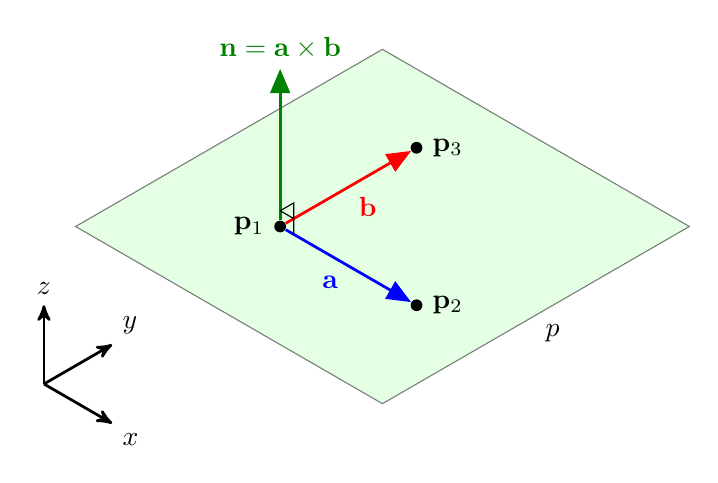
\begin{tikzpicture}
    \coordinate (p1) at (3,2);
    \coordinate (p2) at ($(p1)+(330:2)$);
    \coordinate (p3) at ($(p1)+(30:2)$);
    \coordinate (O) at (0, 0);
    \draw [axis] (O) -- ++(-30:1) node [below right] {$x$};
    \draw [axis] (O) -- ++(30:1) node [above right] {$y$};
    \draw [axis] (O) -- ++(90:1) node [above] {$z$};
    \draw [black,fill=green!20,opacity=0.5] ($(p1)+(330:-1.5)+(30:-1.5)$) -- ++(330:4.5) -- node [below right,black,opacity=1] {$p$} ++(30:4.5) -- ++(150:4.5) -- cycle;
    \node [point,label={180:$\mathbf{p}_1$}] (p1) at (p1) {};
    \node [point,label={0:$\mathbf{p}_2$}] (p2) at (p2) {};
    \node [point,label={0:$\mathbf{p}_3$}] (p3) at (p3) {};
    \draw [bluevec] (p1) -- (p2) node [pos=0.5,below left] {$\mathbf{a}$};
    \draw [redvec] (p1) -- (p3) node [pos=0.5, below right] {$\mathbf{b}$};
    \draw [greenvec] (p1) -- ++(90:2) node [above] {$\mathbf{n} = \mathbf{a} \times \mathbf{b}$};
    \draw ($(p1)+(90:0.2)$) -- ++(30:0.2) -- ++(270:0.2);
    \draw ($(p1)+(90:0.2)$) -- ++(330:0.2) -- ++(270:0.2); 
\end{tikzpicture}

% Shortest distance between a point and a line
% \tikzmath{\a1=10;}
% \begin{tikzpicture}
%     \coordinate (p) at (0, 0);
%     \coordinate (r) at ($(p)+(\a1:3)$);
%     \coordinate (q) at ($(r)+(\a1+90:2)$);
%     \draw ($(p)+(\a1-180:2)$) -- ($(p)+(\a1:5)$) node [left,pos=0,black] {$\ell$};
%     \node [point,label={270:$\mathbf{p}$}] (p) at (p) {};
%     \node [point,label={below:$\mathbf{q}$}] (r) at (r) {};
%     \node [point,label={above:$\mathbf{r}$}] (q) at (q) {};
%     \draw [bluevec] (p) -- (r) node [pos=0.5,below] {$\mathbf{d}$} ;
%     \draw [redvec] (r) -- (q);
%     \draw ($(r)+(\a1-180:0.2)$) -- ++(\a1+90:0.2) -- ++(\a1:0.2);
%     \draw [dblarrow] ($(r)+(\a1:0.2)$) -- node [right] {$d$} ($(q)+(\a1:0.2)$);
% \end{tikzpicture}

% Shortest distance between two lines
% \begin{tikzpicture}
%     \coordinate (O1) at (0,0);
%     \coordinate (O2) at (0,3);
%     \coordinate (Q1) at (0,0);
%     \coordinate (Q2) at (0,3);
%     \coordinate (P1) at ($(Q1)+(-1.5,0)$);
%     \coordinate (P2) at ($(Q2)+(160:1.5)$);
%     \draw [green,fill=green!20,opacity=0.3] ($(O1)+(345:-2)+(30:-1.5)$) -- ++(345:4) -- ++(30:3) -- ++(165:4) -- ++(210:3);
%     \draw [blue,fill=blue!20,opacity=0.3] ($(O2)+(345:-2)+(30:-1.5)$) -- ++(345:4) -- ++(30:3) -- ++(165:4) -- ++(210:3);
%     \begin{scope}
%         \clip (1,0) ($(O1)+(345:-2)+(30:-1.5)$) -- ++(345:4) -- ++(30:3) -- ++(165:4) -- ++(210:3);
%         \draw ($(O1)+(180:4)$) -- ++(0:8) node [above,pos=0.75,black] {$\ell_1$};
%     \end{scope}
%     \begin{scope}
%         \clip (1,0) ($(O2)+(345:-2)+(30:-1.5)$) -- ++(345:4) -- ++(30:3) -- ++(165:4) -- ++(210:3);
%         \draw ($(O2)+(160:4)$) -- ++(340:8) node [above,pos=0.7,black] {$\ell_2$};
%     \end{scope}
%     \node [point,label={270:$\mathbf{q}_1$}] at (Q1) {};
%     \node [point,label={90:$\mathbf{q}_2$}] at (Q2) {};
%     \node [point,label={270:$\mathbf{p}_1$}] at (P1) {};
%     \node [point,label={270:$\mathbf{p}_2$}] at (P2) {};
%     \draw (Q1) -- (Q2);
%     \draw ($(Q1)+(0:0.2)$) -- ++(90:0.2) -- ++(0:-0.2);
%     \draw ($(Q2)+(340:-0.2)$) -- ++(270:0.2) -- ++(160:-0.2);
%     \draw [bluevec, blue, line width=1pt] (Q1) -- ++(90:1.5) node [left,pos=0.5] {$\hat{\mathbf{n}}$};
%     \draw [bluevec, red, line width=1pt] (P1) -- (Q1) node [pos=0.5, below] {$\mathbf{d}_1$};
%     \draw [bluevec, green!75!black, line width=1pt] (P2) -- (Q2)node [pos=0.5, above] {$\mathbf{d}_2$};
% \end{tikzpicture}

% Distance between a point an a plane
% \begin{tikzpicture}
%     \draw [line width=1pt] (-3, 0) -- (3, 0) node [pos=0,below] {$p$};
%     \node [point,label=270:$\mathbf{p}$] (p) {};
%     \node [point,label=0:$\mathbf{q}$] (q) at (2, 2) {};
%     \draw [greenvec] (p) -- ++(90:3) node [left] {$\mathbf{n}$};
%     \draw [bluevec] (p) -- (q);
%     \draw [dblarrow] (-0.2, 0) -- node [left] {$d$} ++(0, 2);
%     \draw (0, 2) -- (q) (0,1.8) -- ++(0:0.2) -- ++(90:0.2);
%     \draw (45:1) arc (45:90:1);
%     \node at (67.5:0.67) {$\theta$};
% \end{tikzpicture}

% Linear transformation
% \begin{tikzpicture}
%     % \draw [step=0.5, black!20] (-1,-1) grid ++(7, 5);
%     \draw [blue!40] (-1,-1) grid ++(7, 5);
%     \begin{scope}
%         \clip (-1, -1) rectangle ++(7, 5);
%         \foreach \i in {-5, -4, ..., 5}{
%             \draw [red!40,line width=1pt] (2.5 * \i - 0.5, -1) -- ++(5,10);
%             \draw [red!40,line width=1pt] (-1, 1.67 * \i - 0.33) -- ++(15,5);
%         }
%     \end{scope}
%     \draw [bluevec] (0,0) -- node [below] {$\mathbf{e}_1$} (1,0);
%     \draw [bluevec] (0,0) -- node [left] {$\mathbf{e}_2$} (0,1);
%     \draw [redvec] (0,0) -- node [below right,pos=0.67] {$T(\mathbf{e}_1)$} (3,1);
%     \draw [redvec] (0,0) -- node [above left,pos=0.67] {$T(\mathbf{e}_2)$} (1,2);
%     \fill [red!40,opacity=0.3] (0, 0) -- ++(3, 1) -- ++(1, 2) -- ++(-3, -1) -- cycle;
%     \fill [blue!40,opacity=0.3] (0, 0) rectangle ++(1, 1);
%     \node [point,blue,label={45:\textcolor{blue}{$(1,1)$}}] at (1, 1) {};
%     \node [point,red,label={right:\textcolor{red}{$T\begin{pmatrix} 1\\ 1 \end{pmatrix}$}}] at (4, 3) {};
% \end{tikzpicture}

% Translation
% \begin{tikzpicture}
%     \draw [axis] (0, 0) -- ++(330:2) node [below right] {$x$};
%     \draw [axis] (0, 0) -- ++(30:2) node [above right] {$y$};
%     \draw [axis] (0, 0) -- ++(90:2) node [above] {$z$};
%     \node [point,label=below:$\mathbf{u}$] (u) at (1,2) {};
%     \node [point,label=below:$\mathbf{v}$] (v) at ($(u)+(3,1)$) {};
%     \draw [bluevec] (u) -- (v) node [above,pos=0.5] {$\mathbf{t}$};
% \end{tikzpicture}


% Rotation
% \tikzmath{\a1=20; \a2=60; \l1=4; \l2=1;}
% \begin{tikzpicture}
%     \draw [axis] (0, 0) -- ++(5, 0) node [below] {$x$};
%     \draw [axis] (0, 0) -- ++(0, 4) node [left] {$y$};
%     \node [point, blue] at (\a1:\l1) (1) {};
%     \node [point, red] at (\a2:\l1) (2) {};
%     \draw [bluevec] (0, 0) -- (1) node [pos=0.75,below] {$\mathbf{u}$};
%     \draw [redvec] (0, 0) -- (2) node [pos=0.6,left] {$\mathbf{v}$};
%     \draw [bluevec] (0, 0) -- (0:\l1) node [pos=0.75,below] {$|\mathbf{u}|\mathbf{e}_1$};
%     \draw [bluevec] (0, 0) -- (0:1) node [pos=0.5,below] {$\mathbf{e}_1$};
%     \draw [-latex',red] (\a1:\l2) arc (\a1 : \a2 : \l2);
%     \draw [-latex',blue] (0:{\l2+0.5}) arc (0 : \a1 : {\l2+0.5});
%     \node [red] at ({0.5 * (\a1+\a2)}: {0.75*\l2}) {$\theta$};
%     \node [blue] at ({0.5 * \a1}: {1.2*\l2}) {$\phi$};
%     \draw [blue] (1) -- ({\l1 * cos(\a1)}, 0);
%     \draw [red] (2) -- ({\l1 * cos(\a2)}, 0);
%     \draw [blue] ({\l1 * cos(\a1)-0.2}, 0) -- ++(0, 0.2) -- ++(0.2, 0);
%     \draw [red] ({\l1 * cos(\a2)-0.2}, 0) -- ++(0, 0.2) -- ++(0.2, 0);
% \end{tikzpicture}

% 3D rotation
% \begin{tikzpicture}
%     \draw [axis] (0, 0) -- ++(330:4) node [below right] {$x$};
%     \draw [axis] (0, 0) -- ++(30:4) node [above right] {$y$};
%     \draw [axis] (0, 0) -- ++(90:4) node [above] {$z$};
%     \node [rotate=-30] at (330:5) {
\includegraphics[width=1cm]{../eye.png}};
%     \node [rotate=30] at (30:5) {
\includegraphics[width=1cm]{../eye.png}};
%     \node [rotate=90] at (90:5) {
\includegraphics[width=1cm]{../eye.png}};
%     \draw[line width=2pt,red, -latex',rotate around={60:(330:2.5)}] (330:2.5) [partial ellipse=-80:260:1cm and 0.5cm];
%     \draw[line width=2pt,green!50!black, latex'-,rotate around={-60:(30:2.5)}] (30:2.5) [partial ellipse=-80:260:1cm and 0.5cm];
%     \draw[line width=2pt, blue, -latex',rotate around={180:(90:2.5)}] (90:2.5) [partial ellipse=-80:260:1cm and 0.5cm];
% \end{tikzpicture}

% Rotation about centre
% \begin{tikzpicture}
%     \coordinate (O1) at (0,0);
%     \coordinate (O2) at (5,0);
%     \coordinate (O3) at (10,0);
%     \coordinate (c1) at (2, {(3+sqrt(3))/3});
%     \node[isosceles triangle,isosceles triangle apex angle=60,draw,rotate=90, fill=blue!20,minimum size=1.73cm,opacity=0.25] at (c1) {};
%     \node[isosceles triangle,isosceles triangle apex angle=60,draw,rotate=90, fill=blue!20,minimum size=1.73cm,opacity=0.25] at ($(O2)+(c1)$) {};
%     \node[isosceles triangle,isosceles triangle apex angle=60,draw,rotate=90, fill=blue!20,minimum size=1.73cm,opacity=0.25] at ($(O3)+(c1)$) {};
%     \node[isosceles triangle,isosceles triangle apex angle=60,draw,rotate=90, fill=blue!20,minimum size=1.73cm,opacity=0.75] at (O1) {};
%     \node[isosceles triangle,isosceles triangle apex angle=60,draw,rotate=90, fill=blue!20,minimum size=1.73cm,opacity=0.25] at (O2) {};
%     \node[isosceles triangle,isosceles triangle apex angle=60,draw,rotate=135, fill=blue!20,minimum size=1.73cm,opacity=0.75] at (O2) {};
%     \node[isosceles triangle,isosceles triangle apex angle=60,draw,rotate=135, fill=blue!20,minimum size=1.73cm,opacity=0.25] at (O3) {};
%     \node[isosceles triangle,isosceles triangle apex angle=60,draw,rotate=135, fill=blue!20,minimum size=1.73cm,opacity=0.75] at ($(O3)+(c1)$) {};
%     \node [point,label=below:$\mathbf{c}$] at (c1) {};
%     \node [point,label=below:$\mathbf{c}$] at ($(O3)+(c1)$) {};
%     \draw [bluevec] (c1) -- node [below right] {$-\mathbf{c}$} (O1);
%     \draw [bluevec] (O3) -- node [above left] {$\mathbf{c}$} ++(c1);
%     \foreach \x in {0, 5, 10}{
%         \draw [axis] (\x,0) -- ++(0:3) node [right] {$x$};
%         \draw [axis] (\x,0) -- ++(90:3) node [above] {$y$};
%     }
%     \node at ($(O1)+(2,-1.5)$) {translate by $-\mathbf{c}$};
%     \node at ($(O2)+(2,-1.5)$) {rotate about origin};
%     \node at ($(O3)+(2,-1.5)$) {translate by $\mathbf{c}$};
% \end{tikzpicture}

% Rotation about line
% \tikzmath{\a1=20;}
% \begin{tikzpicture}
%     \coordinate (l) at (2,0);
%     \coordinate (p) at ($(l)+(\a1:1)$);
%     \coordinate (c) at ($(p)+(\a1:4)$);
%     \draw [axis] (0,0) -- (330:2) node [below right] {$x$};
%     \draw [axis] (0,0) -- (30:2) node [above right] {$y$};
%     \draw [axis] (0,0) -- (90:2) node [above] {$z$};
%     \draw [red] (l) -- ++(\a1:6);
%     \node [point,blue,label=below right:\color{blue}$\mathbf{p}$] at (p) {};
%     \draw [bluevec] (p) -- ++(\a1:3) node [pos=0.5,below right] {$\mathbf{d}$};
%     \draw[line width=1pt,red,-latex',rotate around={{\a1+90}:(c)}] (c) [partial ellipse=-80:260:0.5cm and 0.25cm];
% \end{tikzpicture}

% \tikzmath{\a1=20;}
% \begin{tikzpicture}
%     \coordinate (l) at ($(0,0)+(\a1:-1)$);
%     \coordinate (p) at (0,0);
%     \coordinate (c) at ($(p)+(\a1:4.5)$);
%     \draw [axis] (0,0) -- (330:2) node [below right] {$x$};
%     \draw [axis] (0,0) -- (30:2) node [above] {$y$};
%     \draw [axis] (0,0) -- (90:2) node [above] {$z$};
%     \draw [red] (l) -- ++(\a1:6);
%     \draw [bluevec] (p) -- ++(\a1:3) node [pos=1,above] {$\mathbf{d}$};
%     \draw[line width=1pt,red,-latex',rotate around={{\a1+90}:(c)}] (c) [partial ellipse=-80:260:0.5cm and 0.25cm];
%     \draw[line width=1pt,blue,-latex',rotate around={180:(90:1.25)}] (90:1.25) [partial ellipse=-80:260:0.5cm and 0.25cm];
%     \draw [help lines] (\a1:3) -- node [above,rotate=-90] {$d_z$} ++(270:1)
%         ($(\a1:3)+(270:1)$) -- node [below] {$d_1$} (0,0) 
%         ($(\a1:3)+(270:1)$) -- node [pos=0.4,above,rotate=-30] {$d_x$} ++(150:1.6)
%         -- (0,0) node [pos=0.5,above,rotate=30] {$d_y$};
%     \draw [help lines] (30:1.45) -- ++(330:0.2) -- ++(30:0.2);
%     \node [gray] at (15:0.67) {$\phi$};
% \end{tikzpicture}

% \tikzmath{\a1=47;}
% \begin{tikzpicture}
%     \coordinate (l) at ($(0,0)+(\a1:-1)$);
%     \coordinate (p) at (0,0);
%     \coordinate (c) at ($(p)+(\a1:4.5)$);
%     \draw [axis] (0,0) -- (330:2) node [below right] {$x$};
%     \draw [axis] (0,0) -- (30:2) node [below right] {$y$};
%     \draw [axis] (0,0) -- (90:2) node [above] {$z$};
%     \draw [red] (l) -- ++(\a1:6);
%     \draw [bluevec] (p) -- ++(\a1:3) node [pos=0.8,below right] {$\mathbf{d}$};
%     \draw[line width=1pt,red,-latex',rotate around={{\a1+90}:(c)}] (c) [partial ellipse=-80:260:0.5cm and 0.25cm];
%     \draw[line width=1pt,blue,-latex',rotate around={60:(330:1.25)}] (330:1.25) [partial ellipse=-80:260:0.5cm and 0.25cm];
%     \draw [help lines] (\a1:3) -- node [above,rotate=25] {$d_1$} ++(210:2.4);
%     \node [gray,left] at (90:0.5) {$d_z$};
%     \node [gray,rotate=\a1,below] at (\a1:1.5) {$|\mathbf{d}|$};
%     \draw [help lines] (90:0.8) -- ++(30:0.2) -- ++(90:0.2);
%     \node [gray] at ({(\a1 + 90)/2}:0.67) {$\psi$};
% \end{tikzpicture}

% \tikzmath{\a1=90;}
% \begin{tikzpicture}
%     \coordinate (l) at ($(0,0)+(\a1:-1)$);
%     \coordinate (p) at (0,0);
%     \coordinate (c) at ($(p)+(\a1:4.5)$);
%     \draw [axis] (0,0) -- (330:2) node [below right] {$x$};
%     \draw [axis] (0,0) -- (30:2) node [below right] {$y$};
%     \draw [axis] (0,0) -- (90:2) node [left] {$z$};
%     \draw [red] (l) -- ++(\a1:5);
%     \draw [bluevec] (p) -- ++(\a1:3) node [pos=0.5,below right] {$\mathbf{d}$};
%     \draw[line width=1pt,red,-latex',rotate around={{\a1+90}:(90:3.5)}] (90:3.5) [partial ellipse=-80:260:0.5cm and 0.25cm];
% \end{tikzpicture}

% Aeroplane example
% \begin{tikzpicture}
%     \tikzmath{\a1=290;}
%     \coordinate (c) at (60:3);
%     \draw [axis] (150:2) -- (330:4) node [right] {$x$};
%     \draw [axis] (210:2) -- (30:4) node [right] {$y$};
%     \draw [axis] (270:2) -- (90:4) node [above] {$z$};
%     \draw [bluevec] (c) -- ++(\a1:3) node [pos=0.8,right] {$\mathbf{d}$};
%     \node at ($(c)+(0,-0.1)$) [rotate={\a1-1}] {
\includegraphics[width=2cm]{../plane.png}};
%     \node [point,label=above right:$\mathbf{c}$] at (c) {};
%     \draw [redvec] (c) -- (0,0) node [left,pos=0.5] {$-\mathbf{c}$};
% \end{tikzpicture}

% \begin{tikzpicture}
%     \tikzmath{\a1=290;}
%     \coordinate (c) at (0,0);
%     \draw [axis] (150:2) -- (330:4) node [right] {$x$};
%     \draw [axis] (210:2) -- (30:4) node [right] {$y$};
%     \draw [axis] (270:2) -- (90:3) node [above] {$z$};
%     \draw [bluevec] (c) -- ++(\a1:3) node [pos=0.8,left] {$\mathbf{d}$};
%     \node at ($(c)+(0,-0.1)$) [rotate={\a1-1}] {
\includegraphics[width=2cm]{../plane.png}};
%     \draw [help lines] ($(c)+(\a1:3)$) -- node [above,rotate=-90] {$d_z$} ++(90:1) -- node [rotate=30,above] {$d_y$} ++(30:1.2) --  node [rotate=-30,above] {$d_x$} (0,0) ($(c)+(\a1:3)+(90:1)$) -- node [above,rotate={\a1+10}] {$d_1$} (0,0);
%     \draw[line width=1pt,red,-latex',rotate around={180:(0,2)}] (0,2) [partial ellipse=-80:260:0.5cm and 0.25cm];
%     \draw [help lines] (330:2.2) -- ++(210:0.2) -- ++(330:0.2);
% \end{tikzpicture}

% \begin{tikzpicture}
%     \tikzmath{\a1=313;}
%     \coordinate (c) at (0,0);
%     \draw [axis] (150:2) -- (330:4) node [right] {$x$};
%     \draw [axis] (210:2) -- (30:4) node [right] {$y$};
%     \draw [axis] (270:2) -- (90:3) node [above] {$z$};
%     \draw [bluevec] (c) -- ++(\a1:3) node [pos=0.8,left] {$\mathbf{d}$};
%     \node at ($(c)+(0,-0.1)$) [rotate={\a1-1}] {
\includegraphics[width=2cm]{../plane.png}};
%     \draw[line width=1pt,red,-latex',rotate around={-60:(30:2)}] (30:2) [partial ellipse=-80:260:0.5cm and 0.25cm];
%     \draw [help lines] (\a1:3) -- node [rotate=-90,above] {$d_z$} ++(90:1);
%     \draw [help lines] (330:2.15) -- ++(270:0.2) -- ++(330:0.2);
%     \node [gray,rotate=330,above] at (330:1.5) {$d_1$};
% \end{tikzpicture}

% \begin{tikzpicture}
%     \tikzmath{\a1=330;}
%     \coordinate (c) at (0,0);
%     \draw [axis] (150:2) -- (330:4) node [right] {$x$};
%     \draw [axis] (210:2) -- (30:4) node [right] {$y$};
%     \draw [axis] (270:2) -- (90:3) node [above] {$z$};
%     \draw [bluevec] (c) -- ++(\a1:3) node [below] {$\mathbf{d}$};
%     \node at ($(c)+(0,-0.1)$) [rotate={\a1-1}] {
\includegraphics[width=2cm]{../plane.png}};
%     \draw[line width=1pt,red,-latex',rotate around={60:(330:2)}] (330:2) [partial ellipse=-80:260:0.5cm and 0.25cm];
% \end{tikzpicture}

% Scaling
% \begin{tikzpicture}
%     \tikzmath{\p1=1.5;\p2=2;\p3=1;\s1=2;\s2=1.75;\s3=2;}
%     \draw [axis] (0,0) -- (330:5) node [right] {$x$};
%     \draw [axis] (0,0) -- (30:5) node [right] {$y$};
%     \draw [axis] (0,0) -- (90:3) node [above] {$z$};
%     \node [point,blue,label=left:$\mathbf{u}$] (p1) at ($(330:\p1)+(30:\p2)+(90:\p3)$) {};
%     \node [point,blue,label=right:$\mathbf{v}$] (p2) at ($(330:\s1*\p1)+(30:\s2*\p2)+(90:\s3*\p3)$) {};
%     \draw [help lines,dblarrow] (330:\p1) -- node [rectangle,fill=white,rotate=30] {$u_y$} ++(30:\p2) ;
%     \draw [help lines,dblarrow] (30:\p2) -- node [rectangle,fill=white,rotate=-30] {$u_x$} ++(330:\p1);
%     \draw [help lines,dblarrow] ($(30:\p2)+(330:\p1)$) -- node [rectangle,fill=white,rotate=-90] {$u_x$} ++(90:\p3);
%     \draw [help lines,dblarrow] (330:\s1*\p1) -- node [rectangle,fill=white,rotate=30] {$s_yu_y$} ++(30:\s2*\p2) ;
%     \draw [help lines,dblarrow] (30:\s2*\p2) -- node [rectangle,fill=white,rotate=-30] {$s_xu_x$} ++(330:\s1*\p1);
%     \draw [help lines,dblarrow] ($(30:\s2*\p2)+(330:\s1*\p1)$) -- node [rectangle,fill=white,rotate=-90] {$s_zu_z$} ++(90:\s3*\p3);
%     \draw [redvec] (p1) -- (p2);
% \end{tikzpicture}

% Scaling about centre
% \begin{tikzpicture}
%     \coordinate (O1) at (0,0);
%     \coordinate (O2) at (5,0);
%     \coordinate (O3) at (10,0);
%     \coordinate (c1) at (2, {(3+sqrt(3))/3});
%     \node[isosceles triangle,isosceles triangle apex angle=60,draw,rotate=90, fill=blue!20,minimum size=1cm,opacity=0.25] at (c1) {};
%     \node[isosceles triangle,isosceles triangle apex angle=60,draw,rotate=90, fill=blue!20,minimum size=1cm,opacity=0.75] at ($(O1)$) {};
%     \node[isosceles triangle,isosceles triangle apex angle=60,draw,rotate=90, fill=red!20,minimum size=2cm,opacity=0.75] at (O2) {};
%     \node[isosceles triangle,isosceles triangle apex angle=60,draw,rotate=90, fill=blue!20,minimum size=1cm,opacity=0.25] at (O2) {};
%     \node[isosceles triangle,isosceles triangle apex angle=60,draw,rotate=90, fill=red!20,minimum size=2cm,opacity=0.25] at (O3) {};
%     \node[isosceles triangle,isosceles triangle apex angle=60,draw,rotate=90, fill=red!20,minimum size=2cm,opacity=0.75] at ($(O3)+(c1)$) {};
%     \node[isosceles triangle,isosceles triangle apex angle=60,draw,rotate=90, fill=blue!20,minimum size=1cm,opacity=0.25] at ($(O3)+(c1)$) {};
%     \node [point,label=below:$\mathbf{c}$] at (c1) {};
%     \node [point,label=below:$\mathbf{c}$] at ($(O3)+(c1)$) {};
%     \draw [bluevec] (c1) -- node [below right] {$-\mathbf{c}$} (O1);
%     \draw [bluevec] (O3) -- node [below right] {$\mathbf{c}$} ++(c1);
%     \foreach \x in {0, 5, 10}{
%         \draw [axis] (\x,0) -- ++(0:3) node [right] {$x$};
%         \draw [axis] (\x,0) -- ++(90:3) node [above] {$y$};
%     }
%     \node at ($(O1)+(1.5,-1.5)$) {translate by $-\mathbf{c}$};
%     \node at ($(O2)+(1.5,-1.5)$) {scale about origin};
%     \node at ($(O3)+(1.5,-1.5)$) {translate by $\mathbf{c}$};
% \end{tikzpicture}


\end{document}